\chapter{Literature Review}\label{ch:LitReview}

\subsection{PLL Taxonomy}
\begin{figure}[!htb]
\centering

\usetikzlibrary{shadows,arrows}
% Define the layers to draw the diagram
\pgfdeclarelayer{background}
\pgfdeclarelayer{foreground}
\pgfsetlayers{background,main,foreground}
 
% Define block styles  
\tikzstyle{materia}=[draw, fill=blue!20, text width=6.0em, text centered,
  minimum height=1.5em,drop shadow]
\tikzstyle{Lab} = [materia, text width=8em, minimum width=10em,
  minimum height=3em, rounded corners, drop shadow]
\tikzstyle{texto} = [above, text width=6em, text centered]
\tikzstyle{linepart} = [draw, thick, color=black!50, -latex', dashed]
\tikzstyle{line} = [draw, thick, color=black!50, -latex']
\tikzstyle{ur}=[draw, text centered, minimum height=0.01em]
 
% Define distances for bordering
\newcommand{\blockdist}{1.3}
\newcommand{\edgedist}{1.5}
\newcommand{\myBlock}[2]{node (p#1) [Lab]{#2}}

% Draw background
\newcommand{\background}[5]{%
  \begin{pgfonlayer}{background}
    % Left-top corner of the background rectangle
    \path (#1.west |- #2.north)+(-0.5,0.5) node (a1) {};
    % Right-bottom corner of the background rectanle
    \path (#3.east |- #4.south)+(+0.5,-0.25) node (a2) {};
    % Draw the background
    \path[fill=yellow!20,rounded corners, draw=black!50, dashed]
      (a1) rectangle (a2);
    \path (a1.east |- a1.south)+(0.8,-0.3) node (u1)[texto]
      {\scriptsize\textit{Unidad #5}};
  \end{pgfonlayer}}

\newcommand{\transreceptor}[3]{%
  \path [linepart] (#1.east) -- node [above]
    {\scriptsize Transreceptor #2} (#3);}

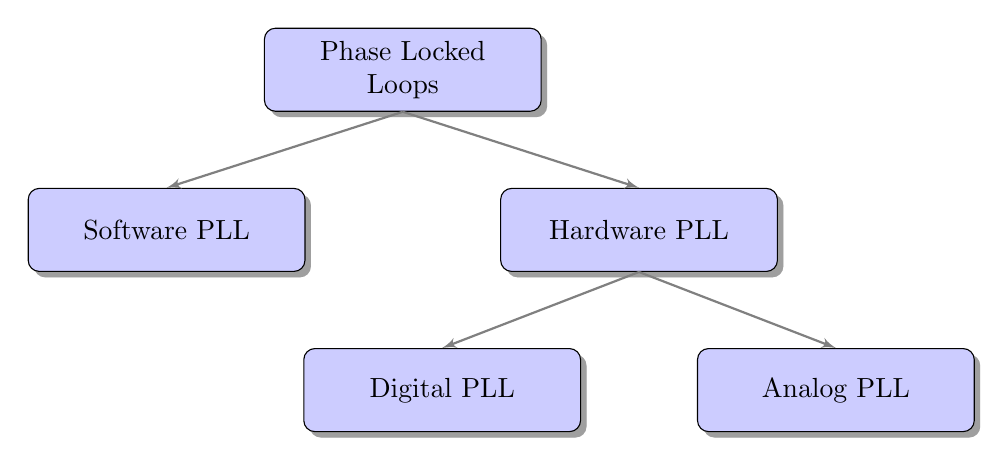
\begin{tikzpicture}[transform shape]
 
 % Draw diagram elements
  \path \myBlock {1}{Phase Locked Loops};
  \path (p1.south)+(-3,-1.5) \myBlock{2}{Software PLL};
  \path (p1.south)+(3,-1.5) \myBlock{3}{Hardware PLL};
  \path (p3.south)+(2.5,-1.5) \myBlock{4}{Analog PLL};
  \path (p3.south)+(-2.5,-1.5) \myBlock{5}{Digital PLL};
     
  % Draw arrows between elements
  \path [line] (p1.south) -- node  {} (p2.north);
  \path [line] (p1.south) -- node  {} (p3.north);
  \path [line] (p3.south) -- node  {} (p4.north);
  \path [line] (p3.south) -- node  {} (p5.north);

\end{tikzpicture}
\caption{A taxonomy of PLLs \cite{Best}}
\label{fig:Taxonomy}
\end{figure}

\begin{table}[!htb]
\centering
\begin{tabular}{|l|l|l|l|}
\hline
\rowcolor[HTML]{C0C0C0} 
\begin{tabular}[c]{@{}l@{}}PLL Category\end{tabular}            & Phase Detector & Phase Error Signal & Loop Filter \\ \hline
\begin{tabular}[c]{@{}l@{}}LPLL (Linear PLL)\end{tabular}       & Analog         & Analog             & Analog      \\ \hline
\rowcolor[HTML]{EFEFEF} 
\begin{tabular}[c]{@{}l@{}}DPLL (Digital PLL)\end{tabular}      & Digital        & Analog             & Analog      \\ \hline
\begin{tabular}[c]{@{}l@{}}ADPLL (All Digital PLL)\end{tabular} & Digital        & Digital            & Digital     \\ \hline
\rowcolor[HTML]{EFEFEF} 
\begin{tabular}[c]{@{}l@{}}SPLL (Software PLL)\end{tabular}     & Software       & Software           & Software    \\ \hline
\end{tabular}
\label{SomeTable}
\caption{\cite{ADPLL},\cite{best2007phase}}
\end{table}


\section{Loop order and Type}
the order is the degree of the denominator of the transfer function. 
Loop type refers to the number of integrators within the loop. A loop with 2 integrators is type 2. The order can never be less than the type. \cite{Gardner}


\section{Jwo}
\cite{Jwo}
However, reduced bandwidth increases
tracking errors due to dynamics. Beyond a certain limit it causes a serious degradation in the
dynamic tracking performance. Therefore, there is involvement of a trade-off between two
opposing considerations: narrow tracking loop bandwidths are desired for filtering noise due to
thermal effects, but wide tracking loop bandwidths are desired to permit tracking of vehicle
dynamics.

The tracking errors of a receiver operating on the GPS code
and carrier include two major components: noise error,
caused by thermal noise; and transient error, caused by
imperfectly tracking the vehicle dynamics.


Either the carrier loop or the code loop is usually
designed to select a bandwidth which produces tracking
errors under maximum dynamics approximately equal to
the lock limit of the loop. When the GPS signal power is
limited, the tendency would seem to make the receiver
tracking-loop bandwidth narrower. However, this increases
the probability that the tracking loop will lose lock owing
to vehicle/user dynamics. Thus, there is a fundamental
system limitation of tracking-loop threshold when considering
both low carrier-to-noise ratio and user dynamics at
the same time. It is therefore important to analyse the error
characteristics for determining the optimal loop bandwidth
that minimises the total tracking error.

The GPS receiver contains a code tracking loop and a
carrier tracking loop for tracking the Doppler-shifted
carrier. The pseudorange obtained from the code tracking
loop provides a position fix; the pseudorange rate estimate
obtained from the carrier tracking loop provides a velocity
fix. The receiver carrier tracking loop is more sensitive to
dynamics due to the fact that it tracks a much higher
frequency signal than a code tracking loop. If the carrier
tracking loop loses lock during a dynamic manoeuvre, the
code tracking loop will usually lose lock subsequently.

Third orders are insensitive
to acceleration, and optimal for constant jerk (rate of change of acceleration) input; fourth-order loops are insensitive
to jerk. It is rare that a loop is constructed with an
order higher than third.

Figure 2

The formula for 

The
C/NO s of the GPS with good signal power typically range
from 35-55 dB-Hz,

The loop order is sensitive to the same order of dynamics,
e.g. first order to velocity stress, second order to acceleration
stress, and third order to jerk stress. The first-order
loop is suitable for a user position that varies in a random
walk manner (white noise velocity); the second-order loop
is suitable for a user velocity that varies in a random walk
manncr (white noise acceleration); the third-order loop is
suitable for a user acceleration that varies in a random walk
manner (white noise jerk).


If the error should become too
large that the VCO skips cycles, the loop is considered to have lost lock.

Diagrams 14a, 14b, 14c 

Compare loop derivation with Kaplan






\section{Xie}

\cite{PengXie}
\subsection{Analog}

\begin{table}[!htb]
\centering
\begin{tabular}{|l|l|}
\hline
\rowcolor[HTML]{C0C0C0} 
Loop Order & Noise Bandwidth as a Function of $\Omega_n$ \\ \hline
First      & $B_n = 0.25 \Omega_n$                       \\ \hline
\rowcolor[HTML]{EFEFEF} 
Second     & $B_n = 0.53 \Omega_n$                       \\ \hline
Third      &  $B_n = 0.7845\Omega_n$                \\ \hline
\end{tabular}
\caption{My caption}
\label{tab:LoopOrderNoiseBandwith}
\end{table}

\begin{table}[!htb]
\centering
\begin{tabular}{|l|l|l|}
\hline
\rowcolor[HTML]{C0C0C0} 
Loop Order & Steady-State Error                                                 & Characteristics                  \\ \hline
First      & $\phi_e = \frac{\Delta f}{\omega_n}$                            & Sensitive to velocity stress     \\ \hline
\rowcolor[HTML]{EFEFEF} 
Second     & $\phi_e = \frac{\Delta \dot{f}}{\omega^2 _n}$  & Sensitive to acceleration stress \\ \hline
Third      & $\phi_e = \frac{\Delta \ddot{f}}{\omega^3 _n}$ & Sensitive to jerk stress         \\ \hline
\end{tabular}
\caption{where $\Delta f$ is the phase rate.}
\label{tab:NoIdea}
\end{table}


Correlated phase errors on the other hand, include the stochastic errors in the satellite clock, the local oscillator errors when generating the NCO local replica, platform vibration, and dynamic stress due to platform motion.


A FLL-assisted-PLL scheme is used to improve the pull-in ability of the loop filter, as well as reduce the locking time (Ward et al 2006).

In a standard receiver architecture, generally speaking, the carrier loop starts with acquisition, then transitions to a FLL, then to a FLL-assisted-PLL, and finally to a PLL. This is because the FLL is more robust to noise than PLL. Moreover, a FLL
can tolerate higher receiver dynamics (Jwo 2001, Chiou 2004).


For a tracking loop, it is desirable that the transition process (transient response) to be sufficiently fast and damped (Ogata 1997). In GNSS tracking loops, the most widely used loop filters are second-order or third-order filters. For a second-order loop, the transition process is determined by the loop's damping ratio and natural frequency. There is always a trade-off in the design procedure of the damping ratio and natural frequency. A relatively small natural frequency will provide excellent noise performance but will be unable to track dynamics induced on the signal, and also the transition time will be large. In contrast, a relatively large natural frequency will reduce the transition time but will have poor noise performance (Chiou 2004, Gebre-Egziabher et al 2003).



Usually tracking loops use fixed natural frequency and damping ratio loop filters. The typical values for natural frequency and damping ratio in the FLL are 10 Hz and 0.707 respectively, and for PLL they are 15 Hz and 0.707 (Petovello et al 2007). An adaptive filter is employed in Sun (2010), Chiou et al (2007), Petovello et al (2007), and Gebre- Egziabher et al (2005), whereas the natural frequency is changed according to the receiver dynamics and signal power, and better frequency and phase tracking qualities are obtained.


After the PRN code and carrier frequency are correlated with a local signal (over a pre-defined integration interval), the in-phase (I) and quadra-phase (Q) correlator outputs are passed to the discriminators (Borre et al 2006). A discriminator defines the type of tracking loop, for a FLL, the discriminator is used to obtain the frequency difference between the received signal and the local replica; for a PLL, the discriminator is used to get the phase error estimate (Ward et al 2006). The phase error is defined as the average phase error over the integration interval.

Page 34 

Put in a chart showing lower noise getting through a lower bandwidth filter

Third-order loop filters have better dynamic tracking performance than first-order and second-order loop filters; however, third-order loop filters are unstable in some scenarios (Gardner 2005). Second-order loop filters are preferred in the low dynamic scenarios, since second-order loop filters are unconditionally stable with any parameters (Gardner 2005). The loop filter design methods are well documented in the literature, e.g. Best
(2004), Gardner (2005), and Borre et al (2006).

Before the carrier phase reacquisition analysis, the performance of a standard receiver after a loss of lock must be assessed first. The carrier loop starts with acquisition after a loss of lock and then consecutively transitions to a FLL, a FLL-assisted-PLL, and finally a PLL. This can be a time consuming process. Below, the effect of different natural frequencies and damping ratios on the transition time is assessed for a general second- order control system, where the nonlinear behaviour of discriminator is not considered

In the GSNRxTM software receiver, a loss of phase lock is declared when the phase lock indicator (PLI) is smaller than 0.5 (30 degrees phase error), when this happens, the receiver transitions to a FLL (O'Driscoll 2008).

With this in mind, the initial frequency error assessment is only necessary in the loss of signal lock case. The frequency error is mainly due to the vehicle dynamics, satellite movement and receiver clock drift after the loss of signal lock. For the frequency error due to the satellite component, the maximum Doppler drift rate is on the order of 0.9 Hz per second (Watson 2005). Assuming a 30 second interval in which the signal is unavailable or too weak to acquire and track (the "loss of lock time"; 30 s is quite long). The Doppler uncertainty due to satellite motion in this case is 27 Hz. For vehicle motion, assuming the line of sight velocity changes by 30 m/s (100 km/h, which is the general


case in a ground-based vehicle scenario) over 30 seconds, the Doppler change is approximately 150 Hz for the GPS L1 signal. Finally, for even relatively poor oscillators,
the frequency stability over 30 seconds is negligible compared to the previous two effects. As such, the total Doppler uncertainty after 30 s is approximately 200 Hz.



Generally, a GNSS receiver contains a code tracking loop and a carrier tracking loop (Ward et al 2006). The code tracking loop is used to get the pseudorange from the satellite to the receiver; on the other hand, the carrier tracking loop is used to get the carrier Doppler and carrier phase. The pseudorange is used to compute the user position and the carrier Doppler is used to compute the user velocity (Spilker 1996).



Tracking loops continuously follow the dynamic of the incoming signal. Carrier tracking loops in GNSS receivers include frequency tracking and phase tracking, which can be performed by frequency lock loops (FLLs) and phase lock loops (PLLs) respectively (Ward et al 2006). PLL also tracks carrier frequencies; however, the tracking requirement is more stringent than FLL. It is very hard to directly track the carrier phase in a GNSS receiver due to the poor frequency pull-in ability of phase tracking loop. The general acquisition procedure is to start from carrier frequency tracking to reduce the Doppler uncertainty and then transition to carrier phase tracking. If the receiver loses track of a satellite, an acquisition process must be performed again to reacquire the satellite (Gardner 2005).


A tracking loop is a feedback system that tracks the frequency or phase of a received signal. The basic purpose of a FLL (PLL) is to generate a signal whose frequency (frequency and phase) approximates the frequency (frequency and phase) of the received signal (Best 2004). The tracking loop contains three essential elements: a discriminator, a loop filter, and a numerically controlled oscillator (NCO) (Gardner 2005). The signal enters the tracking loop after down-conversion and sampling. After the PRN code and carrier frequency are correlated with a local signal (over a pre-defined integration interval), the in-phase (I) and quadra-phase (Q) correlator outputs are passed to the discriminators (Borre et al 2006). 

The phase error is defined as the average phase error over the integration interval. 

Third-order loop filters have better dynamic tracking performance than first-order and second-order loop filters; however, third-order loop filters are unstable in some scenarios (Gardner 2005). Second-order loop filters are preferred in the low dynamic scenarios, since second-order loop filters are unconditionally stable with any parameters (Gardner 2005). The loop filter design methods are well documented in the literature, e.g. Best
(2004), Gardner (2005), and Borre et al (2006).

The loop filter design methods are well documented in the literature, e.g. Best
(2004), Gardner (2005), and Borre et al (2006).

The carrier loop starts with acquisition after a
loss of lock and then consecutively transitions to a FLL, a FLL-assisted-PLL, and finally
a PLL.

\subsection{Digital}


In the previous sections, the discussions were based on analog systems. In order to
process the digitized data in software receivers, the analog signals must be converted into
discrete signals (Tsui 2004). Generally, FLLs and PLLs are designed by using the analog
methods in the continuous time domain. The digital tracking loops are then derived from
the analog tracking loops


Several techniques can be employed to design the loop filter in
the digital domain; however, the most commonly used method is based on transformation
methods, where the discrete form is obtained by means of mapping functions from the
analog domain.

Note that the transformation methods are effective only when 1 n c B T << , where n B is the
filter noise bandwidth (Ward et al 2006).

\section{Stuff From Namuru}
Before phase lock can be achieved, the frequency of the local signal must be relatively close to frequency of the incoming signal from the satellite. Hence a \ac{FLL} is often used to sufficiently reduce the frequency error between the local signal and the received signal.

The code phase changes with the range to the satellite while the carrier frequency changes around the centre frequency of 1575.42 MHz due to the doppler effect\cite{Tsui}.

The frequency offset due to the \ac{LOS} velocity between the receiver and the satellite can be found as : 

\begin{equation}
\Delta f = f_0\frac{v}{c}
\end{equation}

Where: 
\begin{framed}
\begin{align*}
f_0 &= 1575.42 MHz\\   
c &= 2.99792458 \times 10^8
\end{align*}
\end{framed}

For the GPS L1 \ac{C/A} signal, this results in a shift of 5.25Hz per m/s. 
When the receiver is stationary, there will still be a doppler shift, of up to 20KHz due to the motion of the satellite\cite{Kaplan}. As the receiver moves, there will be an doppler shift due to the change in the \ac{LOS} distance between the satellite and the receiver, resulting in a constant offset, for a constant velocity. If the receiver undergoes a constant acceleration, then the doppler frequency increases as a ramp. The relationship between different derivatives of position, and the doppler frequency produced is in table \ref{table:DopplerDynamics} for reference.

Understanding how the Doppler frequency changes is crucial when designing tracking loops, which shall be discussed in more detail in the literature review. 

A thorough overview of the dynamics experienced during space flight can be found in Appendix 1.
\begin{table}[!htb]
\centering
\begin{tabular}{|l|l|}
\hline
\rowcolor[HTML]{C0C0C0} 
Change in \ac{LOS} Distance & Doppler frequency \\ \hline
Static                 & 0                 \\ \hline
\rowcolor[HTML]{EFEFEF} 
Velocity               & Constant          \\ \hline
Acceleration           & Ramp              \\ \hline
\rowcolor[HTML]{EFEFEF} 
Jerk                   & Parabolic         \\ \hline
\end{tabular}
\caption{The relationship between \ac{LOS} dynamics and Doppler frequency}
\label{table:DopplerDynamics}
\end{table}


The dynamics experienced by the code tracking loop are 1540 times smaller than those experienced by the carrier loop \cite{Kaplan}. Hence the  code loop is significantly more robust than either the \ac{FLL} or \ac{PLL}.

The \ac{PLL} is the most vulnerable of the loops, and under extreme dynamics, the \ac{PLL} will break while the \ac{FLL} will keep tracking, before the \ac{PLL} resumes tracking once the dynamics have subsided to more reasonable levels. If the \ac{PLL} looses phase lock, then the receiver is unable to continue receiving the data signal from the satellite, and hence the receiver is unable to continue providing position solutions. Because of the vulnerability of the \ac{PLL} to dynamics, the analysis and design of \ac{PLL}'s for high dynamics it will be the focus of this thesis. 






\section{Original text}
The theory behind GPS tracking loops has intellectual roots in classical control theory. Ultimately a \ac{GNSS} tracking loop is a control system, attempting to generate a local replica of an incoming signal, with minimal error. Nise \cite{Nise} provides a thorough overview of control theory, while Gardner \cite{Gardner} provides an excellent overview of the operation of PLL, from the viewpoint of classical control theory.  

More recently however, GNSS receiver tracking loop design has evolved in order to meet new challenges, in particular high dynamics and weak signal strength. While high dynamics and weak signal strength may initially appear to be disparate concepts, they are intricately linked through the bandwidth time product($B_LT$). 

The designer of a tracking loop has three different attributes that they can adjust to meet the desired performance 
\begin{enumerate}
\item{Loop architecture}
\item{Loop order}
\item{Loop coefficients}
\end{enumerate}

Of these, the most effort has been expended on determining the optimum loop coefficients. 

\section{Loop architecture}

The choice of architecture strongly determines the overall performance of a \ac{GNSS} receiver, in particular, the architecture must be decided upon with the application of the receiver in mind. To quote Kaplan: 
\begin{quotation}
"There is a paradox that the GPS receiver designer must solve in the design of the pre-detection integration time and the discriminator and loop filter functions of the carrier tracking loop. To tolerate dynamic stress, the pre-detection integration time should be short, the discriminator should be an \ac{FLL}, and the carrier loop filter bandwidth should be wide.

However, for the carrier measurements to be accurate (have low noise), the pre-detection integration time should be long, the discriminator should be a \ac{PLL}, and the carrier loop filter noise bandwidth should be narrow. In practice, some compromise must be made to resolve this paradox."\cite{Kaplan}
\end{quotation}

Ward performs a sophisticated analysis of the trade-off between a \ac{PLL} and a \ac{FLL}, stating that 
\begin{quotation}
"A well-designed frequency lock loop (FLL) will outperform
a well-designed phase lock loop (PLL) tracking threshold
under dynamic stress and RF interference (RFI) conditions.
However, the PLL will significantly outperform the FLL
measurement accuracy."\cite{ward1998}
\end{quotation}

In \cite{ward1998}, an innovative carrier tracking loop design technique which
integrates both the FLL and the PLL characteristics, called an FLL-assisted-PLL is developed. This is the architecture, which can be seen in figure \ref{fig:Architecture} is used in the Namuru receiver, and is further described by Ward in \cite{Kaplan}.

\begin{figure}[!htb] 
    \centering
    \includegraphics[width=1\textwidth]{LitReview/Architecture.png} 
    \caption{The discrete implementation of the Ward architecture (FLL-assisted-PLL). Note that the integrators have been implemented using the bilinear transform \cite{Ward}.}
    \label{fig:Architecture}
\end{figure}

\section{Loop order}
From a careful analysis of control theory, we can gain an understanding of the importance of the loop order on the performance on a tracking loop. Kazemi \cite{KazemiPHD,Kazemi2008} and Gardner \cite{Gardner} both spend a significant amount of time covering the development of a Laplace domain model of a \ac{PLL}. 

Ultimately, a trade-off exists between filter order and stability. First and second order filter are unconditionally stable in the Laplace domain, however they are not as effective as third order loops at coping with dynamics. For example, the residual error of a second order loop is acceleration. This makes it unsuitable for any application where sustained acceleration is likely to be encountered, as the error will increase over time, until phase lock is lost. In most real world scenarios, sustained acceleration is limited, due to limits on maximum achievable velocities. For space based applications however, velocities of thousands of meters per second are routinely achieved. Hence while a second order loop may be suitable for terrestrial applications, a third order loops is required for spaced based applications. 

\begin{table}[!htb]
\centering
\begin{tabular}{|l|l|l|l|}
\hline
\rowcolor[HTML]{C0C0C0} 
Loop order & Filter order & Residual Error & Stability                               \\ \hline
1          & 0            & Velocity       & Stable                                  \\ \hline
\rowcolor[HTML]{EFEFEF} 
2          & 1            & Acceleration   & Stable                                  \\ \hline
3          & 2            & Jerk           & Remains stable at $B_n$ \textless 18 Hz \\ \hline
\end{tabular}
\caption{Loop order behaviour}
\label{table:LoopOrders}
\end{table}

\section{Loop coefficients}

The selection of suitable loop coefficients is the aspect of \ac{PLL} design that has received the most attention in the literature. A number of competing approaches exist, and the state of the art has evolved over time, as \ac{GPS} is applied to new and more challenging applications, in particular high dynamics and weak signal applications.

\subsection{Design in Laplace domain, convert to Z Domain}
A popular method for designing a \ac{DPLL} is to design a \ac{PLL} in the Laplace domain, and then convert it to a \ac{DPLL} using a transform. Examples of analog to digital transformation methods include the bilinear, boxcar and impulse invariant transforms. This method is very common as it results in an a set of easy to follow design equations, which produce tracking loops which are suitable for general use. In the literature, this approach is used by Spilker\cite{Spilker}, Gardner\cite{Gardner}, Kaplan\cite{Kaplan} and Ward\cite{Ward}. In particular, the Ward method of determining loop co-efficients is the one used in the design of the Namuru receiver.

A key advantage of this method is that analysis of the loops can be carried out in the Laplace domain, using tools from classical control theory, for example root locus\cite{Nise}. This is useful, because it provides an understanding of how the stability of the system evolves with changing parameters. 

One of the disadvantages of this procedure, is that the use of a transformation from the Laplace domain to the Z domain results in a filter that is an approximation of the filter in the Laplace domain. If the integration time is sufficiently large, and conversely, the sampling frequency is sufficiently small, then the stability of the filter can be compromised. 

A figure of merit that is useful in comparing the \ac{PLL} designed by a particular method is the product between loop noise bandwidth and integration time ($B_LT$). The concept of the $B_LT$ further re-enforces the ultimate trade-off between integration time (sensitivity) and loop noise bandwidth (dynamics). The maximum stable $B_LT$ achievable by designing in the Laplace domain is approximately 0.4 \cite{Kazemi2008,KazemiPHD}

Finally, it is also important to consider that analogue analysis has made linearising assumptions, and transferring analogue analysis to the digital domain is also non-linear and approximate\cite{Dempster}. 

\subsection{Design by minimising the loop phase jitter}

Kazemi\cite{KazemiPHD,Kazemi2008} provides the most sophisticated analysis of \ac{PLL}. In particular, Kazemi takes into account the effect of averaging and delay, introduced by the integration and dump, allowing stable tracking loops to be developed with large $B_LT$. While Kazemi focuses on the development of receivers for weak signal tracking, his work is still applicable to high dynamics, as increasing the integration time of a receiver for a given noise band with, is equivalent to increasing the noise bandwidth, for a given integration time. 

While the methods described by Kazemi is highly complex, it theoretically offers an order of magnitude improvement in achievable $B_LT$. Kazemi also describes a detailed test plan, for evaluating the performance of the tracking loops, both on real-world and simulated signals, which is very instructive for critically evaluating the performance of new algorithms.
